\chapter{Durchführung der Implementierung}
\section{Implementierungs-Prozess}
Für die Verifikation des Frameworks wird die Matlab-Simulation nach \cite{Olucak.15.02.2017} verwendet. Da es hier lediglich um eine Konvertierung des Codes handelt, werden die mathematischen Modelle nicht explizit erklärt. Vielmehr wird das Vorgehen der Implementierung erläutert, um zu zeigen, wie Programm effizient entwickelt wurde. Gleiches gilt für die Implementierung der Simulationswerkzeuge.\\
 Die Simulations-Umgebung wurde sukzessive aufgebaut. Es wurde stets darauf geachtet, dass nach der Implementierung einer Funktion nach möglich direkt getestet wurde. Erst mit der nachgewiesenen Funktionalität, wurde der nächste Schritt im Prozess durchgeführt. In Abbildung \ref{fig:ImpProzess} wird dieser Prozess dargestellt.
\begin{figure}[h]
	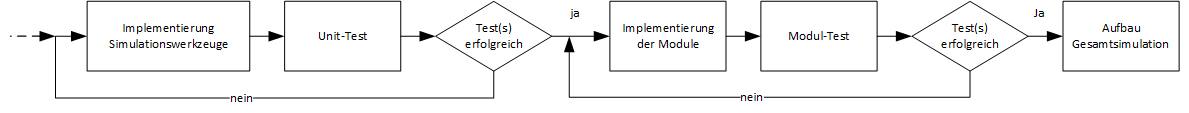
\includegraphics[width=1.0\linewidth]{ImpProzess.PNG}
	\label{fig:ImpProzess}
	\caption{Flussdiagramm des Implementierungs-Prozess}
\end{figure}
\section{Simulationswerkzeuge}
Unter Simulationswerkzeugen sind Funktionen zu verstehen, die in allen Teilen des Simulations-Frameworks vorkommen. Dies umfasst beispielsweise das Einlesen und Schreiben von Simulationsparametern oder mathematische Funktionen wie Integration oder Interpolation. Es ist offensichtlich, dass besagte Funktionen als erstes implementiert werden müssen, damit die Module im späteren Verlauf auf diese zurückgreifen können. Diese Werkzeuge wurden eigens in das Modul \textbf{Tools} implementiert. Auch die in \ref{sec:OSBib} beschriebenen Bibliotheken fallen unter diese Werkzeuge. Die implementierten Simulationswerkzeuge werden in Tabelle \ref{tab: SimWerk} zusammengefasst.
\begin{table}[h]
\centering	\begin{tabular}{lp{11cm}}
		\textbf{Funktion/Klasse} & \textbf{Kurzbeschreibung}\\
		 Constants & physikalische Konstanten\\\\
		 DataLogger & Klassen, um Parameter in ein Text-File zu schreiben\\\\
		 LinearInterpolation & Ein- und zweidimensionale Interpolation bereitstellt\\\\
		 MatFileReader & Funktionen zum Einlesen von .mat-File\\\\
		 ODESolver & Templates für numerische Integration\\\\
		 readInData & Funktionen zum Einlesen von Parametern aus Text-Files\\\\
		 Transformation & Matrizen für Koordinaten-Transformation
	\end{tabular}
\label{tab: SimWerk}
\caption{Simulationswerkzeuge der generischen Flugzeugsimulation}
\end{table}
\newpage
\subsection{Unit-Tests}
Um sicherzustellen, dass die Werkzeuge korrekt implementiert wurden, wurden Unit-Test implementiert. Dazu wurde das in Visual Studio bereitgestellte Microsoft-Komponententest-Frameworks für C++ genutzt. Die Unit-Tests wurden in einen gleichnamigen Projektordner ausgelagert. An dieser Stelle werden nicht alle Test erklärt. Vielmehr soll das Test-Schema erläutert werden.\\ In dieser Arbeit wird das AAA-Schema  (Arrange, Act, Assert) nach \cite{Microsoft.2018}  genutzt. Dazu werden die Tests in die zuvor genannten Abschnitte aufgeteilt. Im einzelnen haben die Abschnitte folgende Bedeutung \cite{Microsoft.2018}: 
\begin{itemize}
	\item  \underline{Arrange} dient der Initialisierung des Tests. Die benötigten Objekte werden initalisiert und Parameter für den Testfall festgelegt.   
	
	\item  Innerhalb von \underline{Act} wird die zu testende Methode mit den zuvor definierten Testfall/Parametern aufgerufen.
	
	\item Im Abschnitt \underline{Assert} werden die Referenzwerte mit den Werten aus dem eigentlichen Test vergleichen. Wird eine Übereinstimmung festgestellt, erhählt der Testfall seine Bestätigung durch das Framework.
\end{itemize}
Die Referenzwerte wurden entweder selbst festgelegt (z.B. Einlesen eines Parameters) oder es wurde Matlab genutzt, um Referenzwerte zu generieren (z.B. Interpolation). \\
Nach \cite{TuxFamily.2018} handelt es sich bei eigen um eine vollständig getestete Bibliothek. Aus diesem Grund wird auf eine Unit-Tests verzichtet. Bei der auf \cite{Hulbert.2013} beruhenden MatFileReader-Klasse wird nur der selbst geschrieben Code getestet. Eine Außnahme bei den Unit-Test stellt das Header-File Constants, bei der lediglich physikalische und mathematische Konstanten hinterlegt sind. 

\section{Implementierung und Testen der Module}
In \ref{sec:AufbauModule} wurde bereits der Aufbau der Module erläutert und in \ref{sec:Ausbaustufen} die für die Simulation benötigten Module aufgelistet. Um die Simulation wie im Baukastenprinzip zusammenzusetzen, ist es erforderlich, dass jedes Teil-Modul korrekt funktioniert.\\
Die Schwierigkeit, die mit den Modul-Tests einhergeht, ist die Definition der Testfälle. Ziel ist es eine größtmögliche Code-Coverage zu haben, um zu garantieren, dass das Modul wie gewünscht funktioniert.Bei einigen Modulen ist das Testen nur bedingt oder  nur im Gesamtsystem-Test möglich. Dies betrifft beispielweise das \textbf{Autopilot} und \textbf{Guidance} Modul. Für beide Module werden Parameter von anderen Modulen benötigt. \\Eine weitere Problematik besteht bei den verschiedenen  Modellen der Ausbaustufen. Wie schon erwähnt, wird die 6 Dof-Simulation nach \cite{Olucak.15.02.2017} genutzt, um das Simulations-Framework zu testen. Somit liegen nur zu den dort verwendeten Modellen Referenzwerte vor. Für die Simulation mit 3 Freiheitsgraden liegt keine Referenz vor. Ähnlich verhält sich die 6 Dof-Simulation mit Fehlermodellen. Es liegen aktuell keine Modelle für Sensorik und Aktuatorik vor. Somit können an dieser Stelle keine Modul-Tests für die zusätzlichen Module erfolgen.
In Tabelle \ref{tab:modultests} werden die Module  und deren Testfälle aufgezeigt, für die ein Modul-Test in Betracht kommt.\\
\begin{table}[h]
\centering	\begin{tabular}{l p{12cm}}
		\textbf{Modul} & \textbf{Beschreibung Testfall}\\
		Atmosphere & Bei dem hier hinterlegten Modell  handelt es sich um die Standard-Atmosphäre von 1976.  Temperatur, Druck, Dichte und Schallgeschwindigkeit sind hierbei abhängig von der Flughöhe. Somit werden die zuvor beschriebenen Größen von 0-10000m berechnet und mit Daten der Standard-Atmosphäre verglichen.\\\\
		Aerodynamic & Hier wird ein Windtunnel bei konstanter Höhe simuliert. Es werden Machzahl, Anstellwinkel und Höhenruder-Winkel variiert. Es ist ersichtlich, dass nur die Längsbewegung betrachtet wird. Dies ist auf mangelnde Referenzwerte für die Seitenbewegung zurückzuführen. Ziel dieses Tests ist es die Polare des Flugzeuges abzufahren und mit den Matlab-Daten zu vergleichen. \\\\
		Autopilot &  Die Parameter für das Gain Scheduling werden eingelesen und die Zustände auf Arbeitspunkt (Trimmpunkt) initialisiert. Es wird überprüft, ob die Scheduling Parameter und Stellgrößen nach der Initialisierung mit denen aus Matlab übereinstimmen.\\\\
		Trajectory & Der Trajectory-Modul Test testet die korrekte Berechnung der Flugbahn. Hier wird die Matlab-Simulation simuliert. Im Anschluss können die Ergebnisse verglichen werden.
	\end{tabular}
\label{tab:modultests}
\caption{Auflistung der Modultests}
\end{table}
\newpage
Aufgrund der Einfachheit des aktuell hinterlegten Schub-Models (Engine-Modul) wurde auf einen Modul-Test verzichtet und der Nachweis über Code-Reading durchgeführt.
Es ist offensichtlich, dass das Trajektorien-Modul erst aufgebaut werden konnte, nachdem die dafür benötigten Module bereits erfolgreich getestet wurden.


\section{Verifikation des Simulations-Framework}
